\begin{frame}{A Taxonomy of Repeated Games Models}
    \begin{figure}
        \tikzstyle{mybox} = [draw=gray!20, fill=white, very thick,
        rectangle, rounded corners, inner sep=10pt, inner ysep=10pt]
        \tikzstyle{fancytitle} = [fill=gray, text=white, rounded corners]
        \scalebox{0.7}{
        \begin{tikzpicture}
            \node [mybox] at (0, 0) (gen-mod){%
                \begin{minipage}{0.50\textwidth}
                    \vspace{-0.25cm}
                    \[ \Gamma^r = (N, \Theta, (D_i, S_i, u_i)_{i\in N}, q, p) \]
                \end{minipage}
            };
            \node [inner sep=0pt] (gen-mod-img) at (-4.4, 0.5){%
                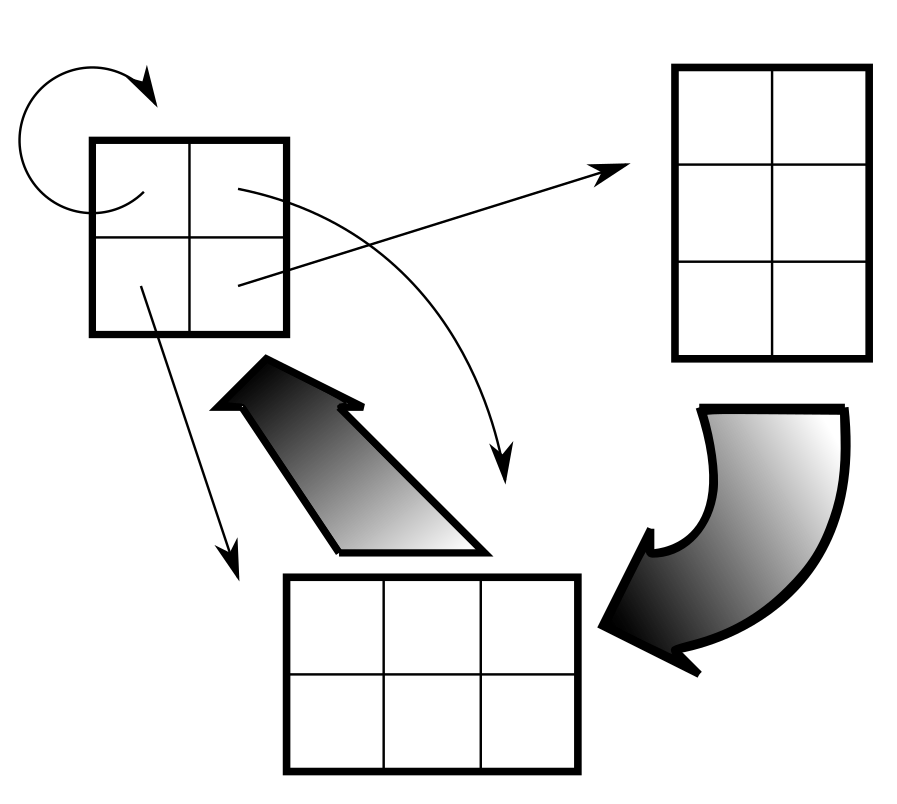
\includegraphics[width=0.25\textwidth]{img/stochastic.png}
            };
            
            \node [mybox] at (-4.5, -3) (mdp){%
                \begin{minipage}{0.40\textwidth}
                    {\color{green}Single-agent stochastic game}
                    \vspace{-0.25cm}
                    \[ |N| = 1. \]
                \end{minipage}
            };
            
            \node [mybox, draw=black] at (0, -7.5) (state){%
                \begin{minipage}{\textwidth}
                    {\color{green}At every round, every player knows the
                    current state of nature $\theta \in \Theta$.} \\
                    Informally, for each player $i \in N$, there exists some
                    state $w(s_i) \in \Theta$ such that the signal $s_i$ can
                    never occur unless the current state is $w(s_i)$.
                \end{minipage}
            };
            
            \node [mybox] at (4.5, -3.5) (std){%
                \begin{minipage}{0.60\textwidth}
                    \begin{itemize}
                        \item {\color{green}Only one possible state of
                        nature}
                        \[ |\Theta| = 1. \]
                        \item {\color{green}Players know all of each other's past
                        moves}
                        \[ S_i = \bigtimes_{j\in N-i} D_j. \]
                    \end{itemize}
                \end{minipage}
            };
            \node [inner sep=0pt] (gen-mod-img) at (7, -5.5){%
                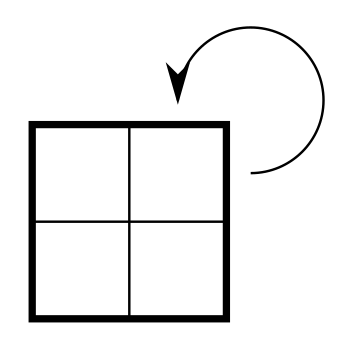
\includegraphics[width=0.20\textwidth]{img/std.png}
            };

            \node[fancytitle] at (gen-mod.north) {Stochastic Games (General Model)};
            \node[fancytitle] at (mdp.north) (mdp-title) {Markov Decision Processes};
            \node[fancytitle, fill=black] at (state.north) (state-title) {Complete State Information};
            \node[fancytitle] at (std.north) (std-title) {Standard Repeated Games};

            \draw[thick, -Latex] (gen-mod.west) -- (mdp-title.north);
            \draw[thick, -Latex] (gen-mod.south) -- (state-title.north);
            \draw[thick, -Latex] (gen-mod.east) -- (std-title.north);
        \end{tikzpicture}}
        \caption{A taxonomy of repeated game models.}
    \end{figure}
\end{frame}

\begin{frame}{Definition : Game with complete state information}

\metroset{block=fill}
\begin{block}{Definition}
A repeated game $\Gamma^r = (N,\Theta, (D_i,S_i,u_i)_{i\in N},q,p)$ has {\color{green}complete state information} if, at every round, every player knows the current state of nature. That is, there is a function $\omega_i:S_i \rightarrow \Theta$ know by each player such that:
\begin{equation*}
    \forall s \in S, \forall \theta, \hat{\theta} \in \Theta, \forall d \in D : p(s,\hat{\theta} | d,\theta) = 0 \text{ if } \hat{\theta} \neq \omega_i(s_i)
\end{equation*}
So the signal $s_i$ can never occur unless the current state is $\omega(s_i)$
\end{block}

\pause
\textbf{\color{green}Is the prisoner's dilemma a game with complete state information?}
\pause

For the prisoner's dilemma, if we assume that \alert{players make decision based only on the last move of their opponent}. We have four different state : $\Theta = \{([C,c]), ([C,d]), ([D,c]), ([D,d])\}$

\end{frame}

\begin{frame}{Definition : stationary}

\metroset{block=fill}
\begin{block}{definition}
In a repeated game, a game is said to be {\color{green}stationary} iff the move probability depends only on the current state. That is there is a function $\tau_i : \Theta \rightarrow \Delta(D_i)$ such that:
\begin{equation*}
	\forall k, \forall s \in (S)^{\times k} : \sigma_i^{[k]}(\cdot | s) = \tau_i(\cdot | \omega_i(s_i^{[k]}))
\end{equation*}
\end{block}

\pause
\textbf{\color{green}Is the grim strategy a stationary strategy?}
\pause

For the prisoner's dilemma, a strategy is said to be stationary, if there is only one move possible for the player at each state $\theta$. The \textbf{grim} strategy depends on past move, and not on the actual state.

\note{
	Explain that this definition is only for game with complete state information
	
	Il faut connaître l'état pour etre stationnaire, si on ne connait pas l'état on ne pourra pas être stationnaire.
}
\end{frame}

\begin{frame}{Small example to understand complete state information}
\textit{Consider the prisoner's dilemma game in a setting where player make decision based only on the last move of they adversary.} \note{This is contrary to decision theory to make this assumption. Some strategies can still be analysed in that setting. (tit-for-tat)}

\pause
$\Rightarrow$ 4 different states : $\Theta = \{([C,c]), ([C,d]), ([D,c]), ([D,d])\}$

\pause
If both player play the \textbf{tit-for-tat} strategy. {\color{green} We can represent } the game like that:

\begin{minipage}{0.7\linewidth}
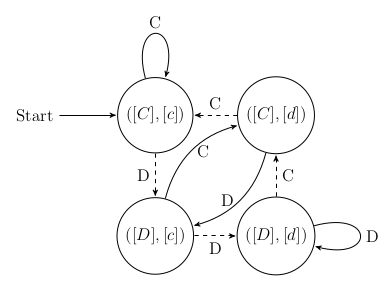
\includegraphics[width=0.9\linewidth]{img/titfortat.png}
\end{minipage}
\begin{minipage}{0.29\linewidth}
	\begin{itemize}
		\item Plain arrow if player 1 play tit-for-tat.
		\item Dashed arrow if player 1 play the opposite.
		\item Player 2 play tit-for-tat
	\end{itemize}
\end{minipage}
\end{frame}

\begin{frame}{How to analyse a game with complete state information ?}
\textbf{Goal of the analyse:} Determine if the game is worth or not .

Let $\nu_i$ be the expected $\delta$-discounted average payoff for player $i$. If player $i$ plan to play a stationary strategy,  and the state of nature at round 1 is $\theta$, the expected $\delta$-discounted average payoff for player $i$ is :
\begin{small}
\begin{eqnarray}
Y_i(\tau, d_i, \nu_i, \theta, \delta) &=&  \sum_{d_i \in D_i} \left( \prod_{j \in N-i} \tau_j(d_j|\theta) \right) \\ && \cdot  \left(  (1-\delta) u_i(d,\theta) + \delta \sum_{\hat{\theta} \in \Theta} \sum_{s \in S} p(s,\hat{\theta} |d,\theta) \nu_i (\hat{\theta}) \right) \label{eq:comp1}
\end{eqnarray}  
\end{small}

\end{frame}


\begin{frame}{Analyze the game with complete state information}
When every players plays according to $\tau$ :

\begin{small}
\begin{align}
\nu_i(\theta, \tau) &=   \sum_{d_i \in D_i} \tau_i(d_i|\theta) \cdot Y_i(\tau, d_i, \nu_i, \theta, \delta)\\
&= \text{max}_{d_i \in D_i} Y_i(\tau, d_i, \nu_i, \theta, \delta) \label{eq:comp2}
\end{align}
\end{small}

\textbf{\color{green} Interpretation}

\begin{itemize}
	\item $Y_i$ is the expected $\delta$-discounted average payoff of player $i$ when the state of nature is $\theta$.
	\item $\tau_i$ is the probability that the move $d_i$ is chosen.
	\item $\Rightarrow$ $\nu_i$ is then the expected $\delta$-discounted average payoff of player $i$ when players plays according to $\tau$
\end{itemize}
\end{frame}

\begin{frame}{Theorem : Equilibrium of the repeated game with standard information}
\metroset{block=fill}
\begin{block}{Theorem 7.1 (numeration from Myreson's book)}
	Given a repeated game with complete state information and bounded payoffs, and given a profile of stationary strategies $\tau$, if there exists a bounded vector $\nu = (\nu_i(\theta))_{\theta \in \Theta, i \in N}$ such that equations (\ref{eq:comp1}) and (\ref{eq:comp2}) are satisfied for every player $i$, then $\tau$ is an equilibrium of the repeated game with the $\delta$-discounted average payoff for player $i$ in the repeated game when the initial state of nature is $\theta$.
\end{block}

\pause


\end{frame}

\begin{frame}{Example with the prisoner's dilemma}
\textit{Consider the prisoner's dilemma where player $i$ plays the \textbf{grim} strategy.}

\pause
We can represent this game with two different state : 
\begin{itemize}
	\item \textbf{1a} : Active plays continuing (Nobody has chosen \textit{defect} in the past)
	\item \textbf{1b} : Active plays continuing (Someone has chosen \textit{defect} in the past)
\end{itemize}

\pause
This strategy is stationary with
$$ \tau_i(c|1a) = 1 \qquad \tau_i(d|1b) = 1$$
\pause
\textbf{\color{green}Using the theorem, compute the value of $\delta$ for which it is not worth to defect.}
\pause

\begin{small}
\begin{align*}
	\nu_i(1a) &= (1-\delta)(-1) + \delta \left( \frac{5}{6} \nu_i(1a) + \frac{1}{6} \nu_i(0) \right) \geq (1-\delta)0 + \delta \left( \frac{5}{6} \nu_i(1b) + \frac{1}{6} \nu_i(0) \right) \\
	\nu_i(1b) &= (1-\delta)(-3) + \delta \left( \frac{5}{6} \nu_i(1b) + \frac{1}{6} \nu_i(0) \right) \geq (1-\delta)(-4) + \delta \left( \frac{5}{6} \nu_i(1b) + \frac{1}{6} \nu_i(0) \right)	\\
	\nu_i(0) &= (1-\delta) 0 + \delta \nu_i(0)
\end{align*}
$$ \Rightarrow \delta \geq \frac{2}{5} $$
\end{small}

\note{
Prisoner's Dilemma in normal form : 
\begin{table}
            \begin{tabular}{c|cc}
                & {\color{red}$a_2$}    & {\color{red}$b2$} \\
                \hline
                {\color{green}$a_1$}    & \payoff{-1}{-1}   & \payoff{-4}{0} \\
                {\color{green}$b_1$}    & \payoff{0}{-4}    & \payoff{-3}{-3} 
            \end{tabular}
            \caption{Prisoner's dilemma in normal form}
        \end{table}
}
\end{frame}

\begin{frame}{Take home message \#}
\metroset{block=fill}
    \begin{block}{Take-home-message \#}
        A {\color{green}repeated game with complete information} is a game where every players know the current state of nature.
        
        A {\color{green}stationary strategy} of a game with complete state information describe the fact that players will play a certain move with probability 1 at in function of the state.
        
        We can observe that some strategies are not stationary at a first sight. But if the players have a $\delta$ big enough, a strategy can become stationary (Cf. grim strategy).
    \end{block}

\end{frame}